\begin{titlepage}
%~\\[1cm]

\begin{minipage}{0.5\textwidth}
\begin{center}
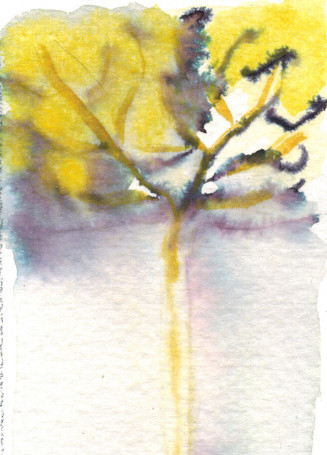
\includegraphics[scale=0.4]{./presentation/gauche}
\end{center}
\end{minipage}
\hfill
\begin{minipage}{0.4\textwidth}
\begin{center}
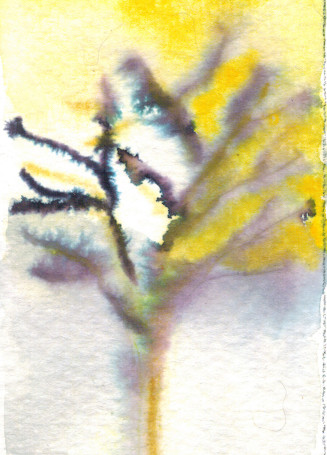
\includegraphics[scale=0.4]{./presentation/droite}
\end{center}
\end{minipage}
\textsc{\Large }\\[0.5cm]

% Title \\[0.4cm]
\HRule

\begin{center}
{\huge \bfseries  Kant\\}
%résumé\\[0.4cm] 
\end{center}

\HRule \\[1.5cm]

\vfill


% Author and supervisor
\begin{minipage}{0.5\textwidth}
\begin{itemize}[leftmargin=1cm, label=\ding{32}, itemsep=2pt]
\item {\bf Objet : } la philosophie de Kant.
\item {\bf Contenu : } extrait d'encyclopédie.
\item {\bf Public concerné : } philosophe en herbe.
\end{itemize}
\end{minipage}
\hfill
\begin{minipage}{0.4\textwidth}
\begin{flushright}% \large
\emph{Numérisation:}\\
Stephan \textsc{Runigo}\\
\emph{Illustration:}\\
\textsc{Krikri}
\end{flushright}
\end{minipage}

\vfill

Ce document est extrait de l'{\it encyclopédie de la philosophie}, {\sc Garzanti}, 2002, et de {\it La pratique de la philosophie}, {\sc Hatier}, 2000.

\vfill

% Bottom of the page
{\large \today}

\end{titlepage}
